\section{Appendix - Design drawings}
\section{Appendix - Model}
\label{AppendixModel}

\subsection{Cross-sections}

\subsection{Hangers}
\label{Appendix_A_Hangers}

\subsection{Live loading} \label{Appendix_Liveloading}
In this chapter, the arrangement of the live loads on the deck is investigated. The three design states ultimate limit state, hanger replacement and hanger loss are treated individually as different circumstances apply to them. In a first step, the location of each lane is defined. The width according to [AASHTO] is always equal to $\SI{12}{ft} = \SI{3.7}{m}$ of which \SI{3}{m} are loaded and the centroid of the applied forces $x_c$ can be derived. The force applied to the tie girder $F_r$ can then be calculated according to Eq. \ref{eq:reaction} using the width of the deck $w_{deck}=\SI{107}{ft}=\SI{32.6}{m}$.
\begin{equation}
    F_r = \frac{x_c}{w_{deck}}
    \label{eq:reaction}
\end{equation}
In a second step, the amount of loaded lanes is determined. As the multiple presence factors (MPF) decrease with the amount of loaded lanes, each possibility is calculated to find the worst arrangement. The calculations are conducted for a unit lane load. The obtained factor relates the load on one lane to the load that is applied on the investigated tie girder. The factor can then be used for the calculation of the force on the tie of the distributed lane load ($q_{LL}=\SI{9.3}{kN/m}$) as well as of the design truck load ($Q_{LL}=\SI{325}{kN}$). For the design truck load an additional dynamic multiplier of 1.33 is taken into account. 

\subsubsection{Characteristic live loading} \label{Appendx_A_Live_loading_1}
In the ultimate limit state, the entire width of the deck is available to traffic. The lanes are arranged as densely to one side as possible and the first lane starts at $\SI{4.6}{ft}=\SI{1.4}{m}$ from the investigated arch plane. The calculations presented in Table \ref{tab:app_ll_uls} show that the worst arrangement results with six loaded lanes. 

\begin{table}[H]
\centering
\begin{tabular}{cccccccccccc}
\cline{2-11}
             & Lane     &  & 1    & 2    & 3    & 4    & 5    & 6    & 7    & 8    &      \\
             & Centroid &  & 2.9  & 6.6  & 10.2 & 13.9 & 17.5 & 21.2 & 24.8 & 28.5 &      \\
             & Reaction &  & 0.91 & 0.80 & 0.69 & 0.57 & 0.46 & 0.35 & 0.24 & 0.13 &      \\ \hline
Loaded Lanes & MPF      &  &      &      &      &      &      &      &      &      & Sum  \\ \hline
1            & 1.2      &  & 1.09 &      &      &      &      &      &      &      & 1.09 \\
2            & 1.0      &  & 0.91 & 0.80 &      &      &      &      &      &      & 1.71 \\
3            & 0.85     &  & 0.77 & 0.68 & 0.58 &      &      &      &      &      & 2.04 \\
4            & 0.75     &  & 0.68 & 0.60 & 0.52 & 0.43 &      &      &      &      & 2.23 \\
5            & 0.70     &  & 0.64 & 0.56 & 0.48 & 0.40 & 0.32 &      &      &      & 2.40 \\
6            & 0.65     &  & 0.59 & 0.52 & 0.45 & 0.37 & 0.30 & 0.23 &      &      & 2.46 \\
7            & 0.60     &  & 0.55 & 0.48 & 0.41 & 0.34 & 0.28 & 0.21 & 0.14 &      & 2.41 \\
8            & 0.55     &  & 0.50 & 0.44 & 0.38 & 0.32 & 0.25 & 0.19 & 0.13 & 0.07 & 2.28 \\ \hline
\end{tabular}
\caption{Force on tie girder for ultimate limit state under unit lane load}
\label{tab:app_ll_uls}
\end{table}

It can be seen that six loaded lanes yield a factor of 2.46. Hence the load applied on the investigated arch plane can be calculated according to Eqs. \eqref{eq:q_ll_uls} and \eqref{eq:Q_ll_uls}. The decisive arrangement is illustrated in Fig. \ref{fig:app_hangers_uls}.
\begin{equation}
    q_{ll, uls} = 2.46 \cdot \SI{9.3}{kN/m} = \SI{22.9}{kN/m}
    \label{eq:q_ll_uls}
\end{equation}
\begin{equation}
    Q_{ll, uls} = 2.46 \cdot 1.33 \cdot \SI{325}{kN} = \SI{1063}{kN}
    \label{eq:Q_ll_uls}
\end{equation}

\begin{figure}[H]
    \centering
    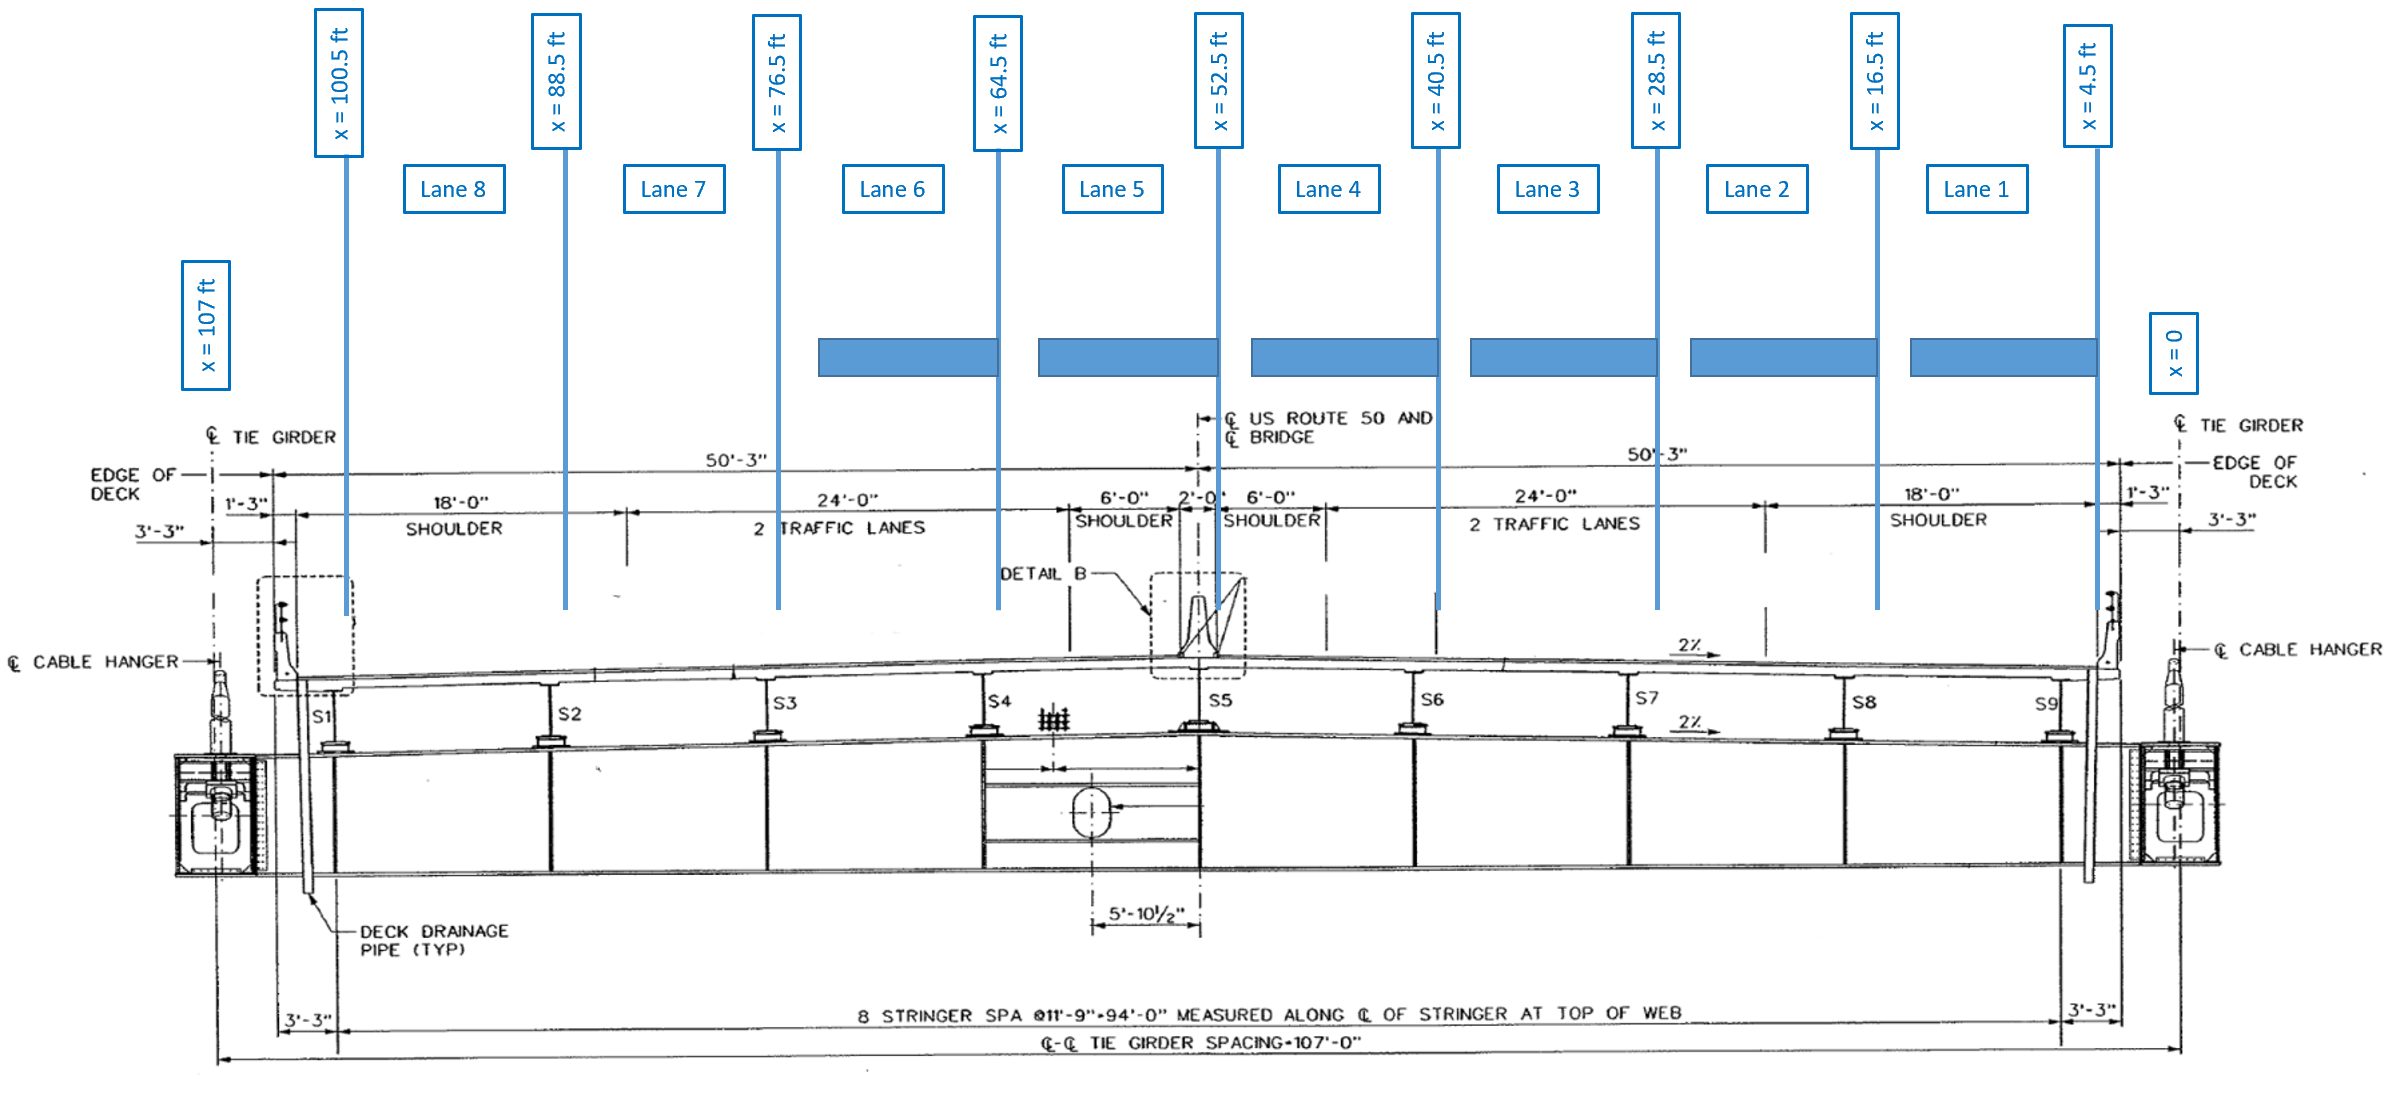
\includegraphics[width=0.9\textwidth]{overleaf/Appendix/Pictures/Cross_Section_LL_ULS.PNG}
    \caption{Live load arrangement in the ultimate limit state}
    \label{fig:app_hangers_uls}
\end{figure}




\subsubsection{Hanger replacement} \label{Appendx_A_Live_loading_2}
In the event of hanger replacement, one lane is shifted away from the hanger being exchanged. Besides that the lanes are located at the same positions as in the ultimate limit state. A load for the replacement truck is disregarded for in this investigation. The calculation of the different arrangements is presented in Table \ref{tab:app_ll_hanger_replacement}.
\begin{table}[H]
\centering
\caption{Force on tie girder for hanger replacement under unit lane load}
\label{tab:app_ll_hanger_replacement}
\resizebox{.8\textwidth}{!}{%
\begin{tabular}{cccccccccccc}
\cline{2-11}
             & Lane     &  & 1    & 2    & 3    & 4    & 5    & 6    & 7    & 8    &      \\
             & Centroid &  & 2.9  & 6.6  & 10.2 & 13.9 & 17.5 & 21.2 & 24.8 & 28.5 &      \\
             & Reaction &  & 0.91 & 0.80 & 0.69 & 0.57 & 0.46 & 0.35 & 0.24 & 0.13 &      \\ \hline
Loaded Lanes & MPF      &  &      &      &      &      &      &      &      &      & Sum  \\ \hline
1            & 1.2      &  & -    & 0.96 &      &      &      &      &      &      & 0.96 \\
2            & 1.0      &  & -    & 0.80 & 0.69 &      &      &      &      &      & 1.49 \\
3            & 0.85     &  & -    & 0.68 & 0.58 & 0.49 &      &      &      &      & 1.75 \\
4            & 0.75     &  & -    & 0.60 & 0.52 & 0.43 & 0.35 &      &      &      & 1.89 \\
5            & 0.70     &  & -    & 0.56 & 0.48 & 0.40 & 0.32 & 0.25 &      &      & 2.01 \\
6            & 0.65     &  & -    & 0.52 & 0.45 & 0.37 & 0.30 & 0.23 & 0.15 &      & 2.02 \\
7            & 0.60     &  & -    & 0.48 & 0.41 & 0.34 & 0.28 & 0.21 & 0.14 & 0.08 & 1.94 \\ \hline
\end{tabular}
}
\end{table}

The resulting loads on the investigated arch plane are presented in Eqs. \eqref{eq:q_ll_repl} and \eqref{eq:Q_ll_repl}
\begin{equation}
    q_{ll, repl} = 2.02 \cdot \SI{9.3}{kN/m} = \SI{18.8}{kN/m}
    \label{eq:q_ll_repl}
\end{equation}
\begin{equation}
    Q_{ll, repl} = 2.02 \cdot 1.33 \cdot \SI{325}{kN} = \SI{874}{kN}
    \label{eq:Q_ll_repl}
\end{equation}

\newpage
\subsubsection{Hanger loss} \label{Appendx_A_Live_loading_3}
In the extreme event of hanger loss, not the entire width of the deck is available to the live loads. For this case, only the four actually marked lanes are available. Their locations were taken from the design drawings. The investigation in Table \ref{tab:app_ll_cable_loss} shows that all of these lanes are loaded in the worst arrangement.
\begin{table}[H]
\centering
\caption{Force on tie girder for cable loss under unit lane load}
\label{tab:app_ll_cable_loss}
\begin{tabular}{cccccccc}
\cline{2-7}
             & Lane     &  & 1    & 2    & 3    & 4    &      \\
             & Centroid &  & 8.4  & 12.0 & 20.0 & 23.6 &      \\
             & Reaction &  & 0.74 & 0.63 & 0.39 & 0.28 &      \\ \hline
Loaded Lanes & MPF      &  &      &      &      &      & Sum  \\ \hline
1            & 1.2      &  & 0.89 &      &      &      & 0.89 \\
2            & 1.0      &  & 0.74 & 0.63 &      &      & 1.37 \\
3            & 0.85     &  & 0.63 & 0.54 & 0.33 &      & 1.50 \\
4            & 0.75     &  & 0.56 & 0.47 & 0.29 & 0.21 & 1.53 \\ \hline
\end{tabular}
\end{table}

The loads resulting on the tie girder are calculated in Eqs. \eqref{eq:q_ll_loss} and \eqref{eq:Q_ll_loss}
\begin{equation}
    q_{ll, loss} = 1.53 \cdot \SI{9.3}{kN/m} = \SI{14.2}{kN/m}
    \label{eq:q_ll_loss}
\end{equation}
\begin{equation}
    Q_{ll, loss} = 1.42 \cdot 1.33 \cdot \SI{325}{kN} = \SI{660}{kN}
    \label{eq:Q_ll_loss}
\end{equation}

An illustration of the load arrangement for the event of cable loss is presented in Fig. \ref{fig:app_hangers_cable_loss}.

\begin{figure}[H]
    \centering
    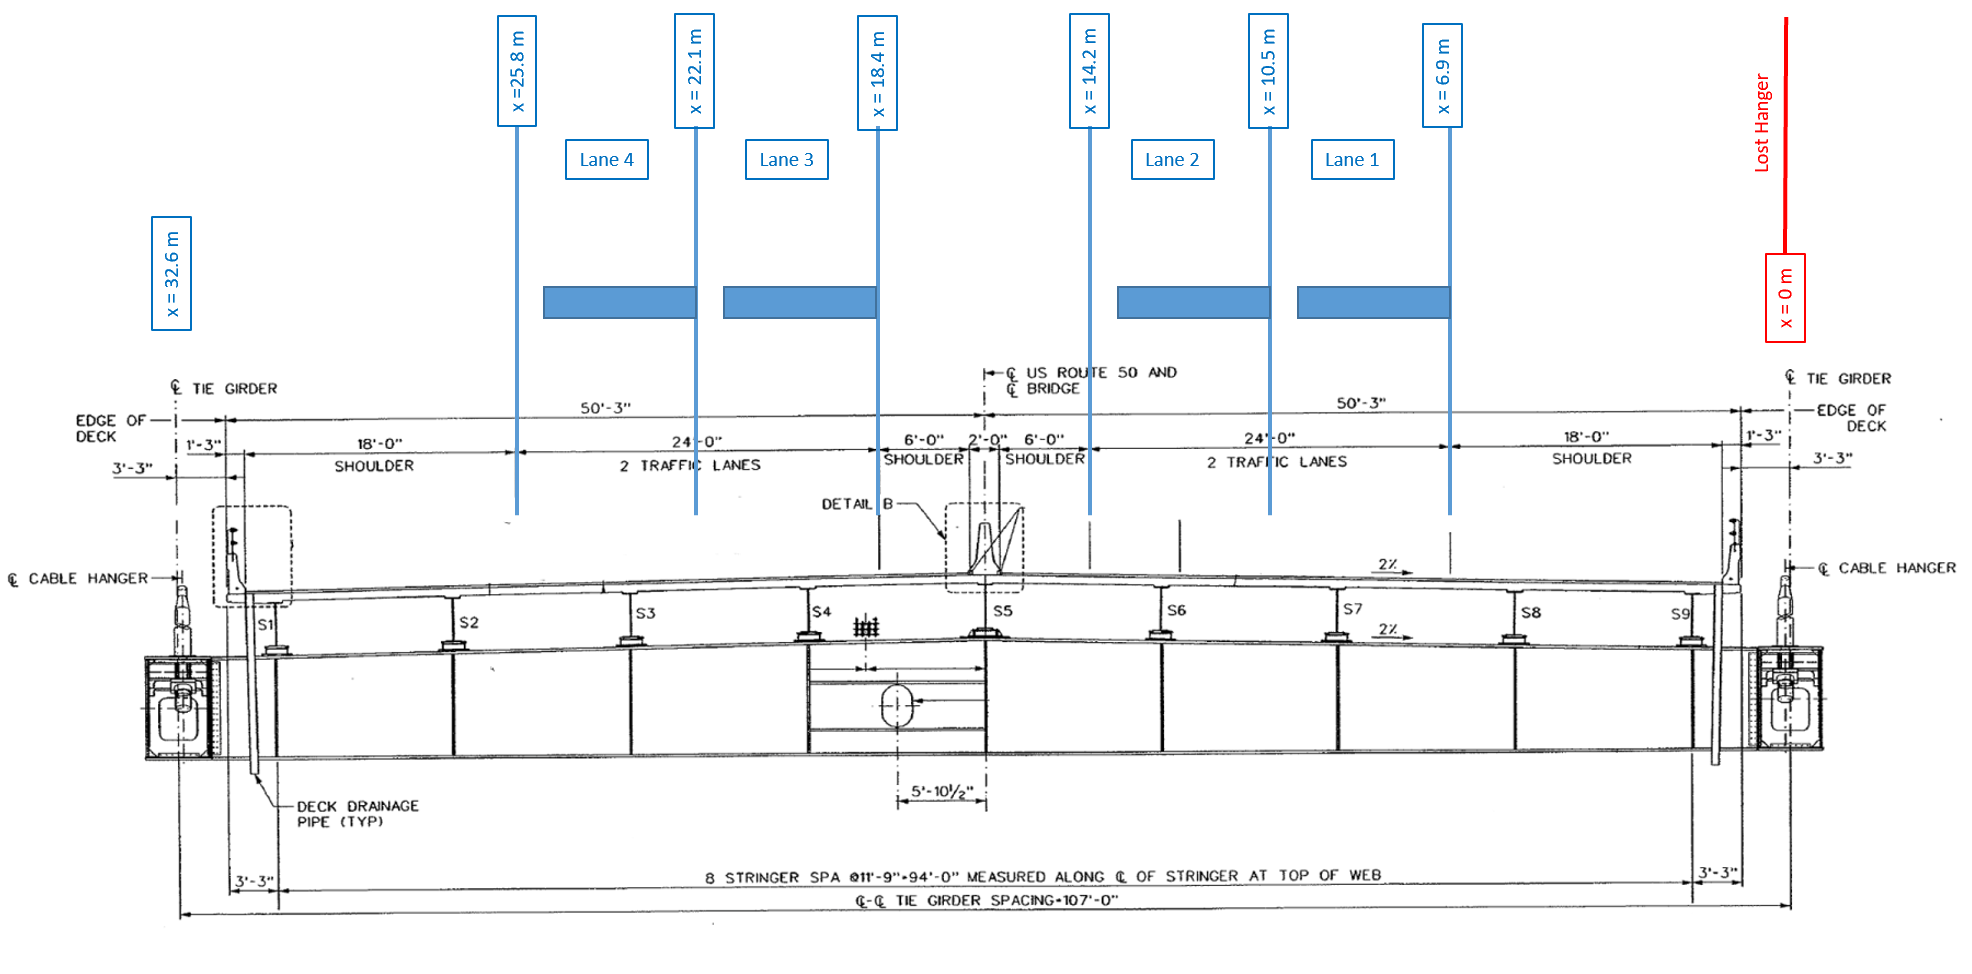
\includegraphics[width=0.9\textwidth]{overleaf/Appendix/Pictures/Cross_Section_LL_Cable Loss.PNG}
    \caption{Live load arrangement for hanger loss}
    \label{fig:app_hangers_cable_loss}
\end{figure}

\newpage
\section{Optimisation methods}
In this chapter, the mathematical background of the used optimisation methods is briefly explained. First, the methods related to the assignment of the permanent hanger forces are introduced in Sec. \ref{app:moment_min} and \ref{app:lsq}. The calculation of the thrust line, including the self weight of the arch, is explained in Sec. \ref{app:thrust_line}.

\subsection{Absolute moment minimisation} \label{app:moment_min}
In a n-times statically indeterminate structure, there are n supernumerary forces or moments. These forces are present in the initial configuration even without any applied loads. The elastic answer of the structure for the different load cases is simply added to obtain the respective effects. It is the goal of an efficient initial configuration to simplify the design verifications by counteracting the effects expected in the various load cases. Here, this is achieved by minimising the permanent moment distribution in the tie and potentially the arch as well. The permanent moment distribution at m points along the considerded component $M \in \mathbb{R}^m$ can be described by Eq. \eqref{eq:perm_mom}. 
\begin{equation}
    {\bf M} = {\bf M_0} + \sum_{i=1}^{n} {\bf M_i} \cdot X_i = {\bf M_0} + {\bf M_{sn}} \cdot {\bf X}
    \label{eq:perm_mom}
\end{equation}
where ${\bf M_0} \in \mathbb{R}^m$ is the moment distribution of the permanent loads on the basic system, ${\bf M_i} \in \mathbb{R}^m$ is the moment distribution of the i-th supernumerary unit force, ${X_i} \in \mathbb{R}$ is the i-th supernumerary force. The later two can be combined into the matrix of supernumerary moments ${\bf M_{sn}} \in  \mathbb{R}^{m\times n}$ and the vector of supernumerary forces or moments ${\bf X} \in \mathbb{R}^n$.

\begin{figure}[H]
\centering
\begin{subfigure}{0.5\textwidth}
    \centering
    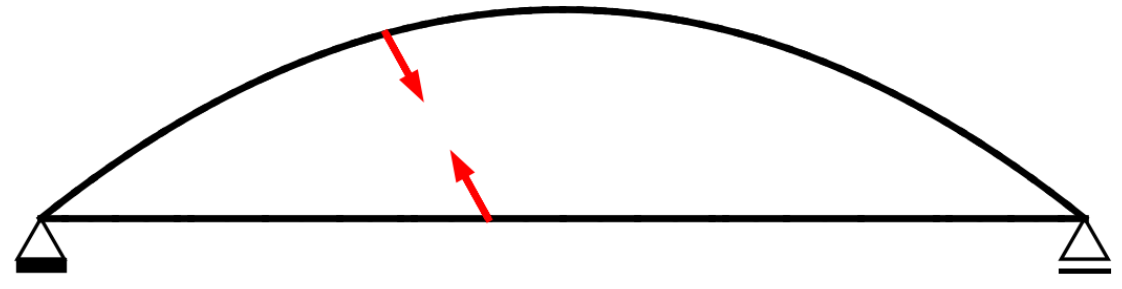
\includegraphics[trim={0 0cm 0 0},clip, width=0.9\textwidth]{overleaf/Appendix/Pictures/min_1.PNG}
    \caption{Basic system and supernumerary force}
    \label{fig:Minimisation_1}
\end{subfigure}%
\begin{subfigure}{.5\textwidth}
    \centering
    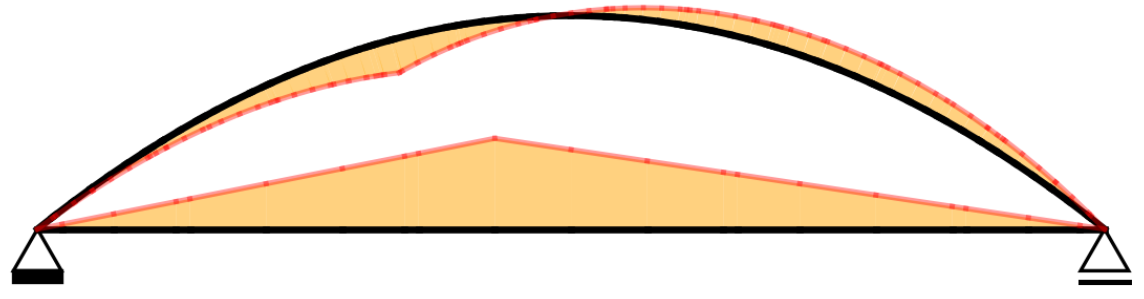
\includegraphics[trim={0 0cm 0 0},clip, width=0.9\textwidth]{overleaf/Appendix/Pictures/min_2.PNG}
    \caption{Moments under supernumerary force}
    \label{fig:Minimisation_2}
\end{subfigure}
\caption{Moment distribution of supernumerary force}
\label{fig:Minimisation}
\end{figure}

The problem of minimising the absolute maximum moments can be formulated according to Eq. \eqref{eq:minimisation}, where the absolute maximum moment is expressed as the infinity norm.
\begin{align}
    \underset{{\bf X}}{\text{Minimize}} \quad & f({\bf X}) = \max({\bf M}, -{\bf M}) = \|{\bf M_0} + {\bf M_{sn}} \cdot {\bf X}\|_{\infty} 
    \label{eq:minimisation}
\end{align}

The helper variable $t$ is introduced, which describes the moment magnitude which is larger than the absolute moments in ${\bf M}$. With the help of $t$, the previously stated problem can be formulated as a linear programming problem, as shown in Eq. \eqref{eq:minimisation_2}.
\begin{align}
    \underset{t, {\bf X}}{\text{Minimize}} \quad & f(t) = t \label{eq:minimisation_2} \\
    \text{s.t.} \quad & {\bf M_0} + {\bf M_{sn}} \cdot {\bf X} - t {\bf 1} \leq  0 \nonumber \\
    \quad & {-\bf M_0} - {\bf M_{sn}} \cdot {\bf X} - t {\bf 1} \leq 0 \nonumber
\end{align}

Additionally, bounds for the permanent hanger forces can be specified as further inequality conditions. It should be noted that under the consideration of symmetry the amount of variables in the linear problem can be reduced. If only the moment distribution in the tie is optimised, it makes sense to only consider vertical forces at each hanger node. In a second step, the optimised vertical forces are assigned to the two hangers at the node.

\subsection{Least squares moments} \label{app:lsq}
As an alternative approach, the supernumerary forces can be determined using the method of least squares. The objective of this method is to find supernumerary forces which counteract a certain moment distribution, for example the moment distribution on the basic system. Using the variables which were introduced in the previous section, the objective is described by Eq. \eqref{eq:lsq_1}.
\begin{equation}
    {\bf M_{sn}} \cdot {\bf X} = -{\bf M_0}
    \label{eq:lsq_1}
\end{equation}
As this yields an overdetermined system, the equations cannot be solved simultaneously. Using the method of least squares, the sum of the squared deviations can be minimised by solving the determined system in Eq. \eqref{eq:lsq_2}.
\begin{equation}
    ({\bf M_{sn}}^T\,{\bf M_{sn}}) \cdot {\bf X} = -{\bf M_{sn}}^T\,{\bf M_0}
    \label{eq:lsq_2}
\end{equation}
The drawback of this method is that no bounds for the hanger forces can be specified. However, this method is particularly useful, if the hanger forces have been optimised by minimising the moments on the tie girder. At this point, the permanent tension force in the tie girder is still undefined, as it does not affect the moment distribution. It can then be calculated by considering the moment distribution in the arch rib, minimising the squares of its moment distribution. In this case, the approach is fast and can even be solved without using linear algebra as there is only one variable.

\subsection{Thrust line derivation} \label{app:thrust_line}

\section{Implementation}

